\documentclass{article}
\usepackage[utf8]{inputenc}
\usepackage{amsmath}
\usepackage{tcolorbox}
\usepackage{amsfonts}
\usepackage{geometry}
\usepackage{pgfplots}
\pgfplotsset{compat=1.16}

\geometry{a4paper, margin=1in}

\title{Statistica e Analisi dei dati}
\author{Matteo Mascherpa}
\date{a.a. 2024/2025}

\begin{document}

\maketitle

\tableofcontents

\section*{Lezione 1}


\section*{Lezione 2}

\section*{Lezione 3}

\section*{Lezione 4}

\section*{Lezione 5}

\section*{Lezione 6}

\subsection*{Mediana Campionaria}

Sia il campione: $23,04,02,2,110,5,7,6,7,3$ la \textit{media campionaria} è $\overline{x} = 140/7=20$. Se si vuole avere un valore che identifichi il centro del campione serve la \textit{mediana campionaria} per indicarla uso $m$.

\begin{tcolorbox}
 Dati i valori di un campione ordinati in ordine crescente. Se la cardinalità del campione è \textbf{dispari} allora $m$ è il valore intermedio della lista altrimenti, se la cardinalità è \textbf{pari} allora $m$ è la media dei due valori intermedi.  
\end{tcolorbox}

Al contrario della \textit{media campionaria} che prende in considerazione tutti i valori degli insiemi dati la \textit{mediana campionaria} non è influenzata dai valori estremi.

\subsection*{Percentili campionari}

La media campionaria è una caso di statistica nota come: \textit{100p-esimo percentile campionario} con $p \in [0,1]$. Esso è un valore che è maggiore del(di almeno) $100p$\% dei valori del campione e minore del(di almeno) $100(1-p)\%$ dei valori. Nel capo della mediana $p=0,5$.

\begin{tcolorbox}
Come trovare il $100p-esimo$ percentile
  \begin{enumerate}
    \item Ordina i dati in ordine crescente
    \item Se $np$ non è intero, trova il più piccolo $\ge$ di $np$. Il valore è quello nella posizione trovata.
    \item Se $np$ è intero, allora il valore è la media tra i valori in posizione $np$ e $np+1$
  \end{enumerate}  
\end{tcolorbox}

\subsection*{Quartili}

I quartili suddividono il campionario dei dati in quattro parti $25\%$ l'una.

\begin{enumerate}
  \item Primo quartile: Il $25$-esimo percentile.
  \item Secondo quartile: Il $50$-esimo percentile.
  \item Terzo quartile: Il $75$-esimo percentile.
\end{enumerate}

\subsection*{Gli insiemi di dati normali e la regola empirica}

La maggior parte degli istogrammi hanno un simile aspetto. Sono spesso simmetrici sulla frequenza massima e assumono una forma a campana. L'insieme di questi istogrammi si dice\textit{istogrammi normali}.  

\begin{tcolorbox}
Un insieme si dice \textit{normale} se il rispettivo istogramma:
\begin{enumerate}
  \item Ha punto di massima in corrispondenza dell'intervallo centrale.
  \item Spostandosi dal centro in una qualsiasi direzione l'altezza cala in modo da creare una forma a campana.
  \item L'istogramma è simmetrico a rispetto all'intervallo centrale.
\end{enumerate}
 
  \textbf{Esempio:} 

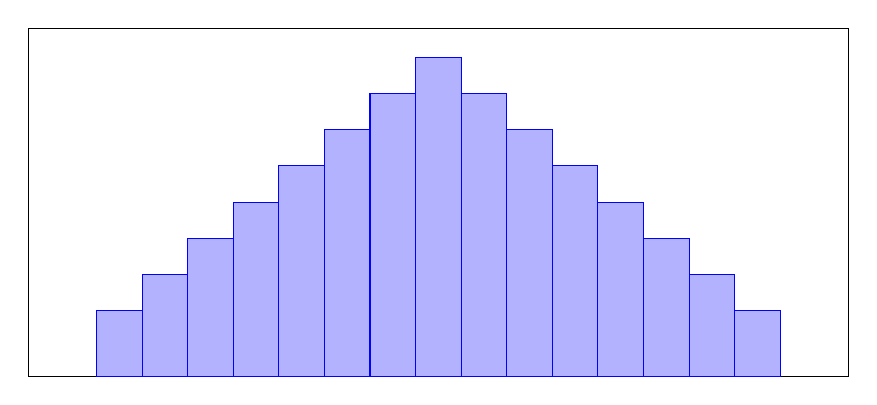
\begin{tikzpicture}
\begin{axis}[
    ybar interval, % Questo specifica che le barre sono intervalli
    width=12cm,
    height=6cm,
    xtick=\empty, % Rimuove i numeri sull'asse x
    ytick=\empty, % Rimuove i numeri sull'asse y
    nodes near coords,
    nodes near coords = \empty 
]
\addplot coordinates {
        (3, 3) (4, 4) (5, 5) (6, 6) (7, 7) (8, 8) (9, 9) 
    (10, 10) (11, 9) (12, 8) (13, 7) (14, 6) (15, 5) (16, 4) (17, 3) 
    (18, 2) 
};
\end{axis}
\end{tikzpicture}

\end{tcolorbox}

\subsection*{Regola empirica}

Se un insieme è approssimativamente normale con media $\overline{x}$ con una devizione standard $s$.

\begin{enumerate}
  \item Approssimativamente $68\%$ dei dati si trovano nell'intervallo: $[\overline{x}-s,\overline{x}+s]$
  \item Approssimativamente $95\%$ dei dati si trovano nell'intervallo: $[\overline{x}-2s,\overline{x}+2s]$
  \item Approssimativamente $99,7\%$ dei dati si trovano nell'intervallo: $[\overline{x}-3s,\overline{x}+3s]$

\end{enumerate}

\hfill

\begin{minipage}[c]{0.35\textwidth}
    \centering
    \begin{tabular}{r|l}
        22 & 372 \\
        23 & 512, 688, 941 \\
        24 & 706 \\
        25 & 020, 057, 128, 400, 446, 575\\
        26 & 183, 894, 982 \\
        27 & 671, 711, 744 \\
        28 & 345, 764, 913, 967 \\
    \end{tabular}
\end{minipage}
\hspace{2mm}
\begin{minipage}[c]{0.6\textwidth}
    \vspace{-2mm}
    Un modo efficiente di rappresentare un insieme di dati di dimensioni medie consiste nell'utizzare il \textit{diagramma ramo-foglia} (o a stelo). Tale grafico si ottiene dividendo ciascun valore dei dati in due parti, chiamati appunto rami e foglie. \\ \\
    La scelta dei rami dovrebbe essere fatta in modo che il \mbox{diagramma} ramo-foglia che ne risulta sia informativo sui dati. Questi diagrammi sono particolarmente adatti a descrivere insiemi di dati dimensioni ridotte.
\end{minipage}

\hfill




\section*{Lezione 7}

\section*{Lezione 8}


\end{document}
